\documentclass[12pt,a4paper]{article}

% Packages
\usepackage[utf8]{inputenc}
\usepackage{graphicx}
\usepackage{amsmath}
\usepackage{hyperref}
\usepackage{geometry}
\usepackage{acronym}
\usepackage{booktabs}
\usepackage{tabularx,ragged2e,booktabs,babel}
\usepackage{lmodern}
\usepackage{microtype}
\usepackage{titlesec}
\usepackage{longtable}
\usepackage[table,xcdraw]{xcolor}
\setcounter{secnumdepth}{4}

\newcommand{\subsubsubsection}[1]{\paragraph{#1}\mbox{}\\}
\setcounter{secnumdepth}{4}
\setcounter{tocdepth}{4}
\titleformat{\paragraph}
{\normalfont\normalsize\bfseries}{\theparagraph}{1em}{}
\titlespacing*{\paragraph}
{0pt}{3.25ex plus 1ex minus .2ex}{1.5ex plus .2ex}
\geometry{margin=1in}

% Title
\title{AAS Type3 - System Architecture}
\author{Ahmed Ibrahim Almohamed}
\date{\today}

\begin{document}

\maketitle



\begin{abstract}
  This document provides a comprehensive overview of the system architecture for the AAS Type3 project. It details the system components, their interactions, and the overall design principles guiding the architecture.
\end{abstract}
\newpage
\tableofcontents

\newpage
\section{System Overview}

\subsection{System Concept}
After reviewing the requirements and doing the necessary research,
a established simple use case was created to illustrate the system concept as in figure \ref{fig:usecase}.

\begin{figure}[h]
    \centering
    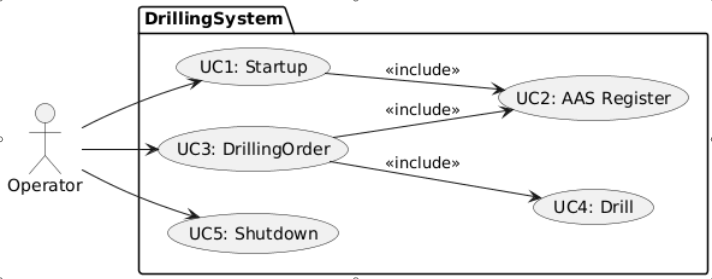
\includegraphics[width=0.8\textwidth]{Images/Usecase.png}
    \caption{System Use Case}
    \label{fig:usecase}
\end{figure}

From the use case and the requirements, the system concept is established where it holds two
main components:
\begin{itemize}
    \item \textbf{An Asset Administration Shell (AAS)}
    \item \textbf{A Run time Environment (RTE) with Multiagent System (MAS)}
\end{itemize}
\begin{figure}[h]
    \centering
    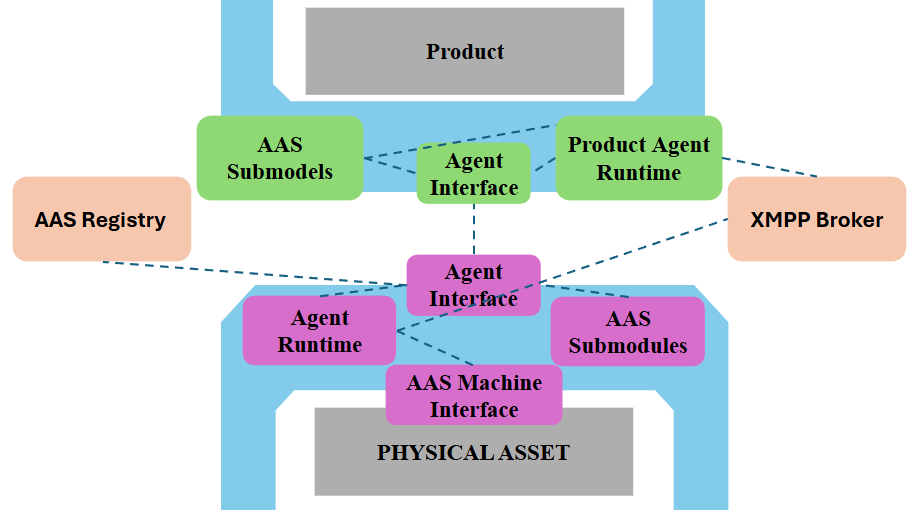
\includegraphics[width=0.8\textwidth]{Images/System_Concept.png}
    \caption{System Concept}
    \label{fig:system_concept}
\end{figure}

The Concept illustrated in figure \ref{fig:system_concept} shows the two main parts , the Product or Production AAS and the Resource AAS.

\subsection{Resource AAS - Overview}
The Resource AAS is the component that describes a resource in the System,
where a Resource in the system can vary from a simple machine to a worker.
The Resource AAS contains the following components:
\begin{itemize}
    \item \textbf{AAS Submodels} that describe the resource properties and capabilities.
    \item \textbf{Agent Runtime} that contains the agent that represents the resource in the system.
    \item \textbf{AgentInterface} that connects the resource Agent to other agents in the system.
    \item \textbf{Agent Machine Interface} that connects the resource Agent to the machine or worker it represents.
\end{itemize}

The Submodels of the Resource AAS contains the following components as in table \ref{table:resource_aas_submodels}.

\begin{table}[h]
\centering
\begin{tabularx}{\textwidth}{>{\raggedright\arraybackslash}X>{\raggedright\arraybackslash}X}
\toprule
\rowcolor[HTML]{38FFF8}
\textbf{Submodel} & \textbf{Description} \\ \midrule
\textbf{Operation State Submodel} & Contains the current operational state of the resource and History. \\
\textbf{Knowledge Submodel} & Contains the knowledge of the resource constraints and the environmental conditions. \\
\textbf{Capabilities Submodel} & Describes the skills the asset can perform and the services it can provide. \\
\textbf{Interaction and scheduling Submodel} & Contains the Communication endpoints and the collaboration mechanisms. \\
\bottomrule
\end{tabularx}
\caption{Resource Agent : Submodels}
\label{table:resource_aas_submodels}
\end{table}
The submodels then could provide the necessary information for the Resource Agent to perform its tasks in the system.
The Resource Agent then connects to other agents in the system through the Agent Interface and to the machine.
As shown in figure \ref{fig:resource_aas_overview}. the Belifes of the agent are updated from the
operational state submodel and the knowledge submodel where they provided the necessary state and constraints for the agent.
The Desires of the agent are established from the capabilities submodel
where they provide the skills and services.
Finaly the agent can act upon the desiers and excute its intention which the scheduling and interaction submodel
can provide the necessary information for the agent to interact and schedule its tasks.
\begin{figure}[h]
    \centering
    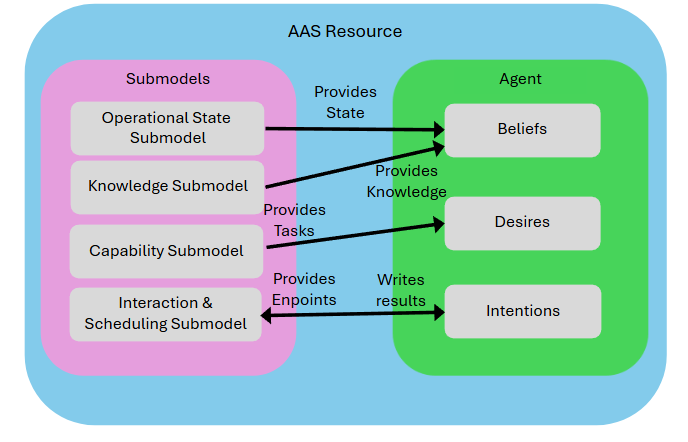
\includegraphics[width=0.8\textwidth]{Images/Resource_Agent_overview.png}
    \caption{Resource AAS Overview}
    \label{fig:resource_aas_overview}
\end{figure}

\newpage
The Resource AAS can interact with other AASs (production or resource).
It also capable of publishing events and subscribing to other AAS events.
As shown in figure \ref{fig:resource_aas_interactions}, the Resource AAS can interact with other AASs through
via XMPP protocol which is a communication protocol for MAS frame work for python \textbf{SPADE}.
XMPP can also be used as a broker for the AAS to publish and subscribe to events.
Finaly the Resource AAS can interact with the Asset via a custom Interface (OPC UA, REST API ...etc).
\begin{figure}[h]
    \centering
    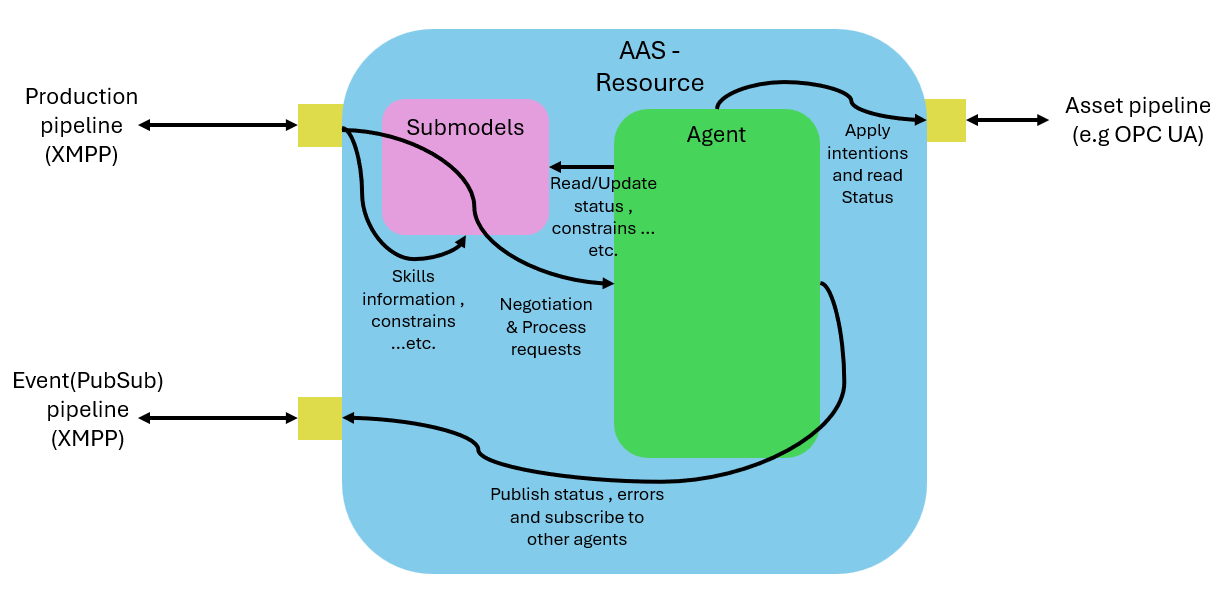
\includegraphics[width=0.99\textwidth]{Images/Resource_Agent_Interaction_Overview.png}
    \caption{Resource AAS Interactions - Overview}
    \label{fig:resource_aas_interactions}
\end{figure}
The communication interfaces and their usage are summarized in table \ref{table:communication_interfaces}.
\begin{table}[h]
\centering
\begin{tabularx}{\textwidth}{>{\raggedright\arraybackslash}X>{\raggedright\arraybackslash}X}
\toprule
\rowcolor[HTML]{38FFF8}
\textbf{Communication Interface} & \textbf{Usage} \\ \midrule
XMPP & Agent-to-agent communication within the MAS framework. \\
XMPP - Events & Publishing and subscribing to events between AASs. \\
Asset Interface (e.g OPC UA) & Interfacing with industrial assets and machines for data exchange and control. \\
\bottomrule
\end{tabularx}
\caption{Communication Interfaces and Their Usage}
\label{table:communication_interfaces}
\end{table}
\newpage
Internally the Submodels are connected to the agent where they could be read and updated.
The Submodels can also provide the production agents with the available services and skills the resource can provide and the state of the resource.
The Agent runtime can connect to the other agents in two ways:
\begin{itemize}
    \item \textbf{Direct Communication} where the agents can communicate directly with each other and hold negotiations.
    \item \textbf{Event-based Communication} where the agents can publish and subscribe to events.
\end{itemize}
Also it handles the execution of the tasks on the machine or worker it represents.

\newpage
\subsubsection{Resource AAS - Architecture Overview }

\begin{figure}[h]
    \centering
    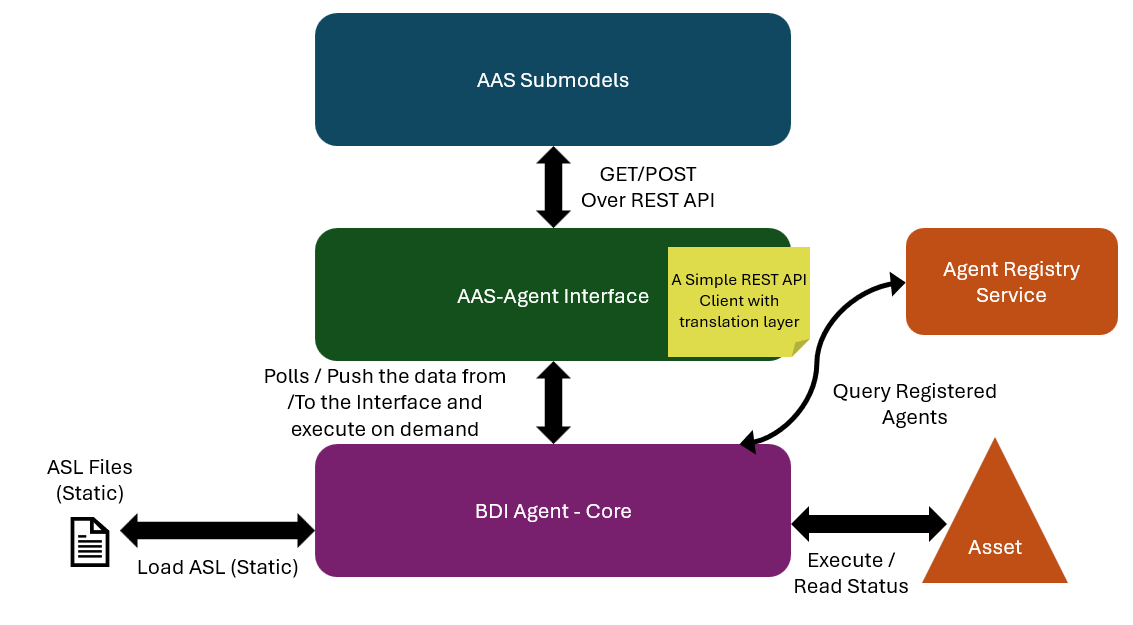
\includegraphics[width=0.99\textwidth]{Images/Resource_Agent_Arch_overview.png}
    \caption{Resource AAS Architecture Overview}
    \label{fig:resource_aas_architecture_overview}
\end{figure}
From an Architecture point of view the Resource AAS can be illustrated as in figure \ref{fig:resource_aas_architecture_overview}.
The overview of the architecture shows three main layers, The \textbf{AAS Submodels} , \textbf{The AAS - Agebnt Interface} and Finaly \textbf{BDI Agent Core}.
The AAS Submodels layer are created via \textbf{Basyx} framework which is an open source framework for creating AASs.
This framework provides the necessary tools to create and manage AASs and their submodels.
It also can provide a REST API for the AAS to be accessed and managed.
The AAS - Agent Interface layer is responsible for connecting the AAS to the Agent Core.
It mainly work as a middleman between the AAS and the Agent Core where it translate the data types of from and to the AAS and the Agent Core.
Finaly The BDI Agent Core is the main component of the Resource AAS where it contains the BDI agent that represents the resource in the system.
The BDI agent is created via \textbf{SPADE} framework which is an open source framework for creating Multi-agent systems in python.
The BDI agent is responsible for managing the beliefs, desires and intentions of the agent.
It also handles the communication with other agents in the system via XMPP protocol.
The BDI agent can also execute the tasks on the machine or worker it represents.
The BDI agent also can register itself with a Agent Registry service that the production Agents
use for discovering the available resources in the system.

\newpage
\subsubsubsection{Submodels with REST API and server}
\begin{figure}[h]
    \centering
    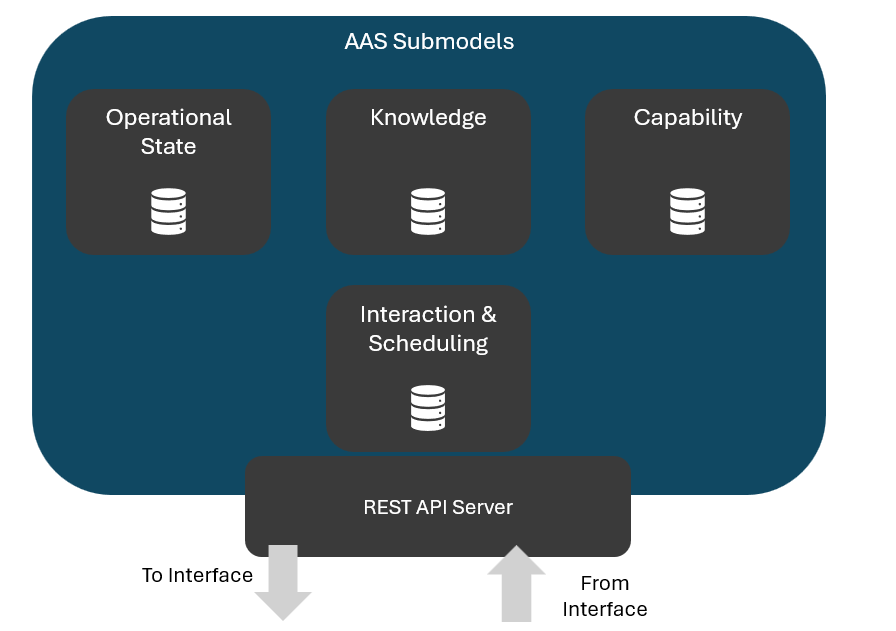
\includegraphics[width=0.8\textwidth]{Images/Resource_Agent_Submodels_Arch_Overview.png}
    \caption{Resource AAS Submodels with REST API and Server}
    \label{fig:resource_aas_submodels_rest_api}
\end{figure}

The Submodels layer as shown in figure \ref{fig:resource_aas_submodels_rest_api} contains the AAS Submodels and a REST API server.
The AAS Submodels are created via \textbf{Basyx} framework which is an open source framework for creating AASs.
This framework provides the necessary tools to create and manage AASs and their submodels.
It also can provide a REST API for the AAS to be accessed and managed.
The Submodels connects to the AAS-Agent Interface via REST API calls where the AAS-Agent Interface can read and update the submodels.

\newpage
\subsubsubsection{AAS-Agent Interface}
\begin{figure}[h]
    \centering
    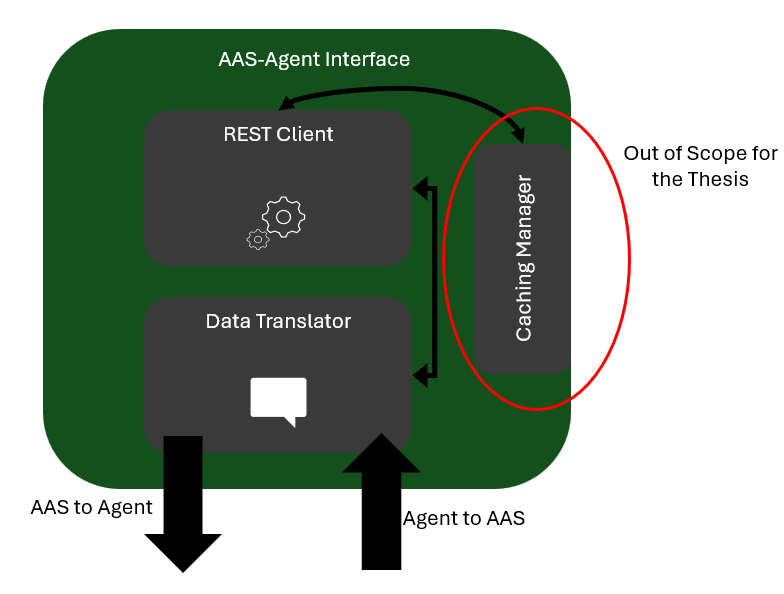
\includegraphics[width=0.9\textwidth]{Images/Resource_Agent_AAS_Agent_interface.png}
    \caption{Resource AAS-Agent Interface}
    \label{fig:resource_aas_agent_interface}
\end{figure}
\\
As in figure \ref{fig:resource_aas_agent_interface} the AAS-Agent Interface is responsible for connecting the AAS to the Agent Core.
It mainly work as a middleman between the AAS and the Agent Core where it translate the data types of from and to the AAS and the Agent Core.
The AAS-Agent Interface contains the following components:
\begin{itemize}
    \item \textbf{REST Client} that connects to the AAS via REST API calls.
    \item \textbf{Data Translator} that translates the data types from and to the AAS and the Agent Core.
\end{itemize}

\newpage
\subsubsubsection{BDI Agent Core}
\begin{figure}[h]
    \centering
    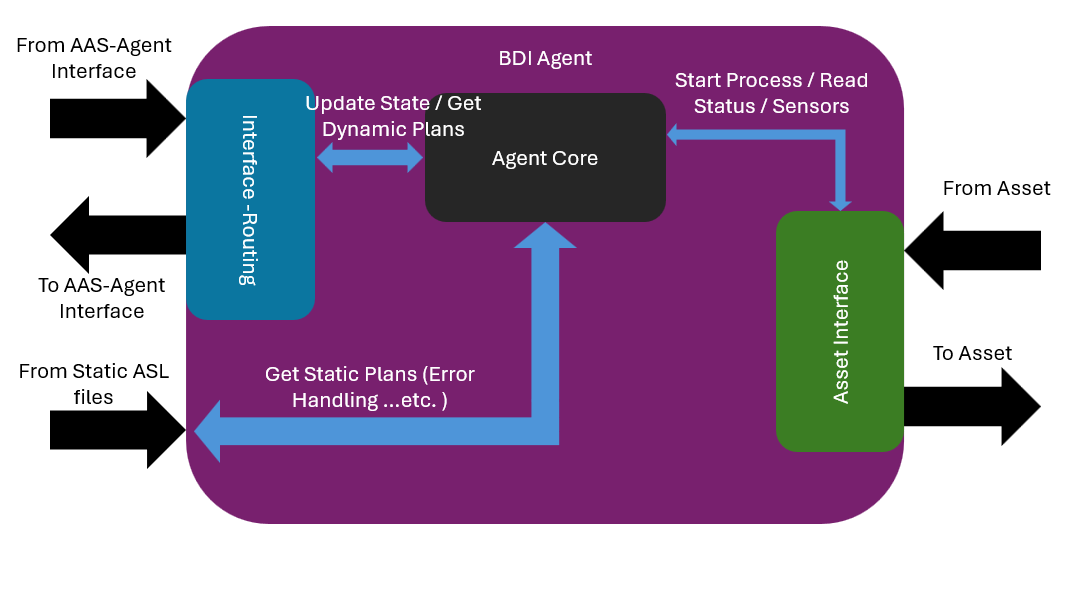
\includegraphics[width=0.99\textwidth]{Images/Resource_Agent_BDI_Overview.png}
    \caption{Resource AAS - BDI Agent Core}
    \label{fig:resource_aas_bdi_agent_core}
\end{figure}
\\
As in figure \ref{fig:resource_aas_bdi_agent_core} the BDI Agent Core is the main component of the Resource AAS where it contains the BDI agent that represents the resource in the system.
The BDI agent is created via \textbf{SPADE} framework which is an open source framework for creating Multi-agent systems in python.
The BDI agent is responsible for managing the beliefs, desires and intentions of the agent.
It also handles the communication with other agents in the system via XMPP protocol.
The BDI agent can also execute the tasks on the machine or worker it represents.
The BDI agent also can register itself with a Agent Registry service that the production Agents
use for discovering the available resources in the system.
The BDI agent contains the following components:
\begin{itemize}
    \item \textbf{Agent Core} that contains the BDI agent and its components.
    \item \textbf{Asset Interface} that connects the agent to the machine or worker it represents.
\end{itemize}
The Agent Core connects with the AAS-Agent Interface so that it can read and update the AAS Submodels.
The Agent Core also connects to other agents in the system via XMPP protocol.
The Agent Core can delegate tasks to the Asset Interface so that it can execute the tasks on the machine or worker it represents.
The Asset Interface connects to the machine or worker via a custom interface (e.g OPC UA, REST API ...etc).

\newpage
\subsection{Production AAS - Overview}

The Production AAS is the component that describes a product in the System,
where a Product in the system can vary from a simple product to a complex assembly.
The Product AAS contains the following components:
\begin{itemize}
    \item \textbf{AAS Submodels} that describe the product properties and capabilities
    \item \textbf{Agent Runtime} that contains the agent that represents the product in the system.
    \item \textbf{AgentInterface} that connects the product Agent to other agents in
\end{itemize}

The Submodels of the Product AAS contains the following components as in table \ref{table:product_aas_submodels}.
\begin{table}[h]
\centering
\begin{tabularx}{\textwidth}{>{\raggedright\arraybackslash}X>{\raggedright\arraybackslash}X}
\toprule
\rowcolor[HTML]{38FFF8}
\textbf{Submodel} & \textbf{Description} \\ \midrule
Identification Submodel  & Contains information about the product ID , version , Owner and Product context\\
Process plan & Contains information about the following : 
\begin{itemize}
    \item Nodes (as task to be performed on the product)
    \item Edges (as the flow between the tasks)
    \item Entry and Exit points
    \item Required Inputs and produced Outputs
    \item Required Capabilities and Skills to perform the tasks
    \item Pre and post conditions for each task
\end{itemize} \\
Services Catalog & Contains information about the services offered by the product, including their capabilities and requirements. \\
Interface and Endpoints & Contains information about the communication endpoints and protocols used by the product. \\
Execution state and Tracking & Contains information about the current state of the product and its history. \\
\bottomrule
\end{tabularx}
\caption{Product AAS Submodels}
\label{table:product_aas_submodels}
\end{table}
\newpage
The submodels then could provide the necessary information for the Product Agent to perform its tasks in the system.
The Product Agent contains an Agent Runtime element that is divied into two cores :
\begin{itemize}
    \item \textbf{The Orchestration Core} that is responsible for managing the overall production process and coordinating the resources.
    \item \textbf{The Negotiation Core} that is responsible for negotiating with the Resource Agents to allocate the necessary resources for the production process.
\end{itemize}
As shown in figure \ref{fig:product_aas_overview}. The Submodels provide the necessary information for the Orchestration Core to manage the production process.
The Orchestration Core gets the ID ,process plan and the Excution state from the Submodels.
It then uses this information to manage the production process and coordinate the resources.
The Orchestration Core then uses the Negotiation Core to negotiate with the Resource Agents to allocate the necessary resources for the production process.
The Negotiation Core then uses the Agent Interface to communicate with the Resource Agents and other Product Agents in the system.
The Submodels also provide the necessary information for the Negotiation Core to negotiate with the Resource Agents.
The Negotiation Core gets the Services Catalog and the Interface , Endpoints from the Submodels and the ID.
\begin{figure}[h]
    \centering
    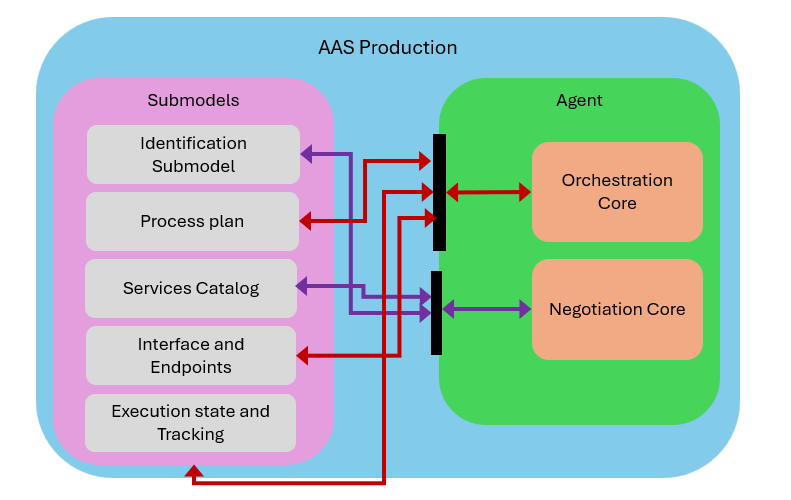
\includegraphics[width=0.9\textwidth]{Images/Production_Agent_overview.png}
    \caption{Product AAS Overview}
    \label{fig:product_aas_overview}
\end{figure}

\newpage
The Product AAS can interact with other AASs (production or resource).
It also capable of publishing events and subscribing to other AAS events.
As shown in figure \ref{fig:product_aas_interactions}, the Product AAS can interact with other AASs through
via XMPP protocol which is a communication protocol for MAS frame work for python \textbf{SPADE}.
XMPP can also be used as a broker for the AAS to publish and subscribe to events.
\begin{figure}[h]
    \centering
    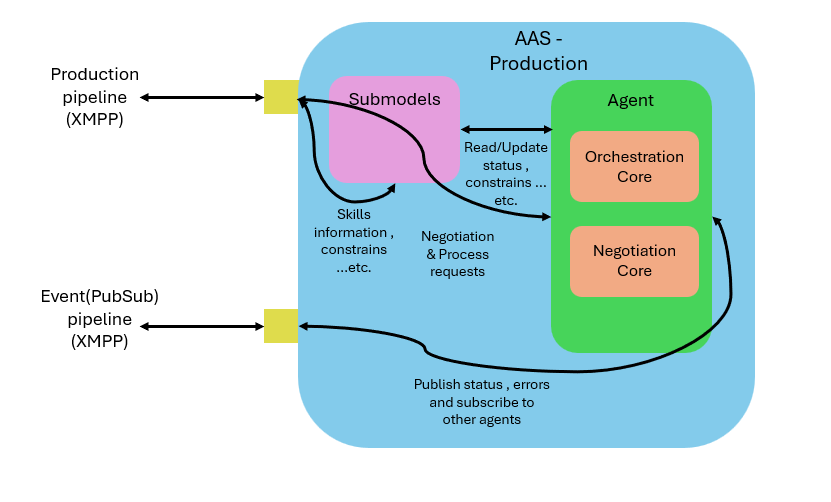
\includegraphics[width=0.99\textwidth]{Images/Production_Agent_Interaction_Overview.png}
    \caption{Product AAS Interactions - Overview}
    \label{fig:product_aas_interactions}
\end{figure}
The communication interfaces and their usage are summarized in table \ref{table:communication_interfaces_product}.
\begin{table}[h]
\centering
\begin{tabularx}{\textwidth}{>{\raggedright\arraybackslash}X>{\raggedright\arraybackslash}X}
\toprule
\rowcolor[HTML]{38FFF8}
\textbf{Communication Interface} & \textbf{Usage} \\ \midrule
XMPP & Agent-to-agent communication within the MAS framework. \\
XMPP - Events & Publishing and subscribing to events between AASs. \\
\bottomrule
\end{tabularx}
\caption{Communication Interfaces and Their Usage - Product AAS}
\label{table:communication_interfaces_product}
\end{table}
\newpage
Internally the Submodels are connected to the agent where they could be read and updated.
The Submodels can also provide the production agents with the process plan and the required services and skills
to perform the production process.
The Orchestration Core can manage the production process and coordinate the resources.
The Negotiation Core can communicate with other agents in the system via XMPP protocol.
The Negotiation Core can also register itself with a Agent Registry service that the Resource Agents
use for discovering the available products in the system.

\newpage
\subsubsection{Product AAS - Architecture Overview }

\begin{figure}[h]
    \centering
    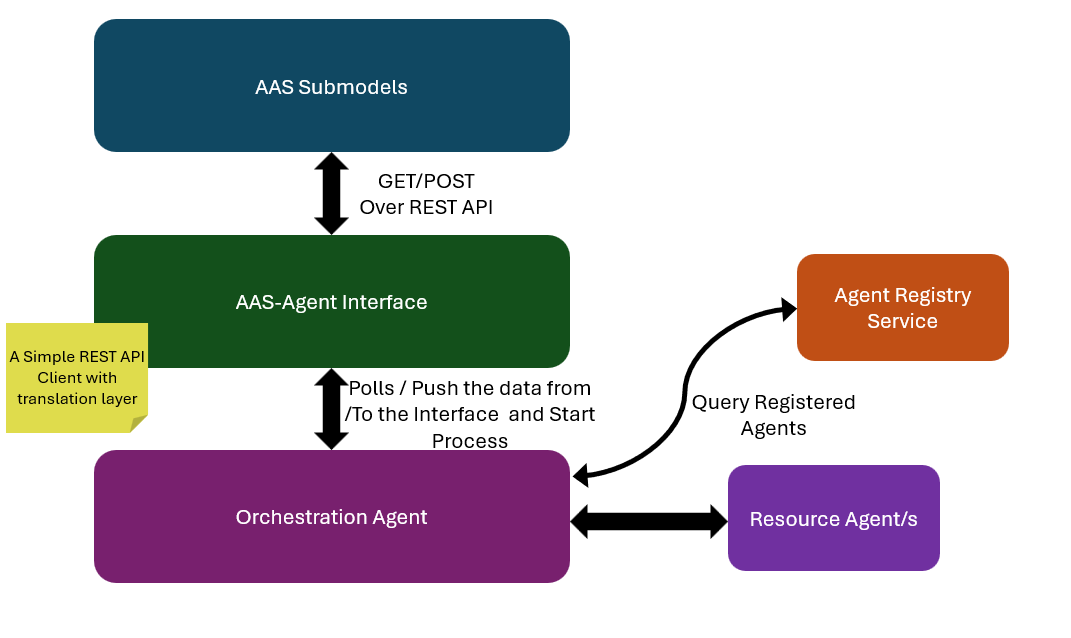
\includegraphics[width=0.99\textwidth]{Images/Production_Agent_Arch_overview.png}
    \caption{Product AAS Architecture Overview}
    \label{fig:product_aas_architecture_overview}
\end{figure}

From an Architecture point of view the Product AAS can be illustrated as in figure \ref{fig:product_aas_architecture_overview}.
The overview of the architecture shows three main layers, The \textbf{AAS Submodels} , \textbf{The AAS - Agent Interface} and Finally  \textbf{Orchestration Agent}.
The AAS Submodels layer are created via \textbf{Basyx} framework which is an open source framework for creating AASs.
This framework provides the necessary tools to create and manage AASs and their submodels.
It also can provide a REST API for the AAS to be accessed and managed.
The AAS - Agent Interface layer is responsible for connecting the AAS to the Orchestration Agent.
It mainly work as a middleman between the AAS and the Orchestration Agent where it translate the data types of from and to the AAS and the Orchestration Agent.
Finally The Orchestration Agent is the main component of the Product AAS where it contains the Orchestration Core and the Negotiation Core that represents the product in the system.
The Orchestration Core and the Negotiation Core are created via \textbf{SPADE} framework which is an open source framework for creating Multi-agent systems in python.
The Orchestration Core is responsible for managing the overall production process and coordinating the resources.
The Negotiation Core is responsible for negotiating with the Resource Agents to allocate the necessary resources for the production process.
The Orchestration Core and the Negotiation Core can also communicate with other agents in the system via XMPP protocol.
The Orchestration Core and the Negotiation Core also can register itself with a Agent Registry service that the Resource Agents
use for discovering the available products in the system.

\newpage
\subsubsubsection{Submodels with REST API and server}
\begin{figure}[h]
    \centering
    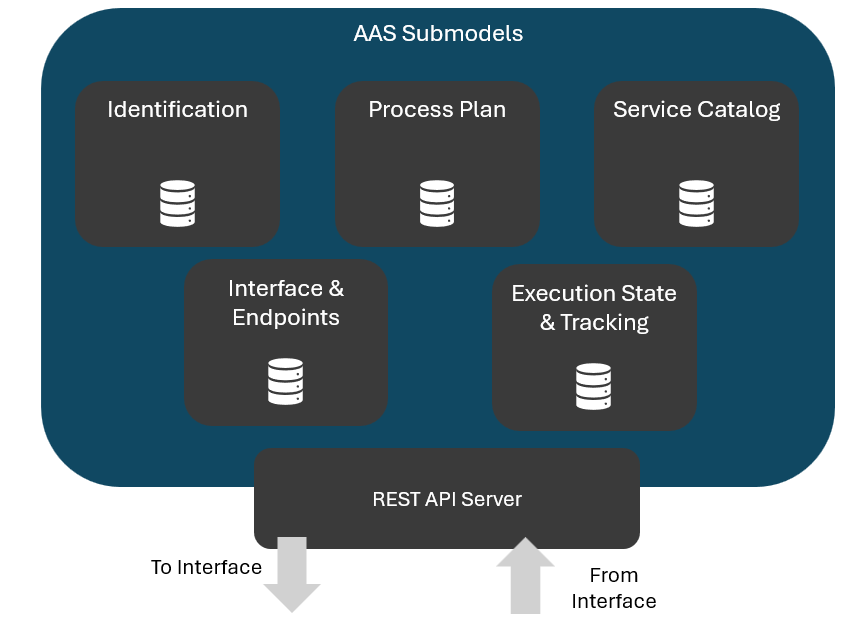
\includegraphics[width=0.8\textwidth]{Images/Production_Agent_Submodels_Arch_Overview.png}
    \caption{Product AAS Submodels with REST API and Server}
    \label{fig:product_aas_submodels_rest_api}
\end{figure}

Similar to the Resource AAS Submodels layer as shown in figure \ref{fig:product_aas_submodels_rest_api} contains the AAS Submodels and a REST API server.
The AAS Submodels are created via \textbf{Basyx} framework which is an open source framework for creating AASs.
This framework provides the necessary tools to create and manage AASs and their submodels.
It also can provide a REST API for the AAS to be accessed and managed.
The Submodels connects to the AAS-Agent Interface via REST API calls where the AAS-Agent Interface can read and update the submodels.

\newpage

\subsubsubsection{AAS-Agent Interface}

Similar to the Resource AAS-Agent Interface as in figure \ref{fig:resource_aas_agent_interface} the Product AAS-Agent Interface is responsible for connecting the AAS to the Orchestration Agent.
It mainly work as a middleman between the AAS and the Orchestration Agent where it translate the data types of from and to the AAS and the Orchestration Agent.
The main diffrence to the Resource AAS-Agent Interface is that it connects to the Orchestration Agent instead of the BDI Agent Core which means the data model to translate is diffrent.
\subsubsubsection{Orchestration Agent and Negotiation Core}

\begin{figure}[h]
    \centering
    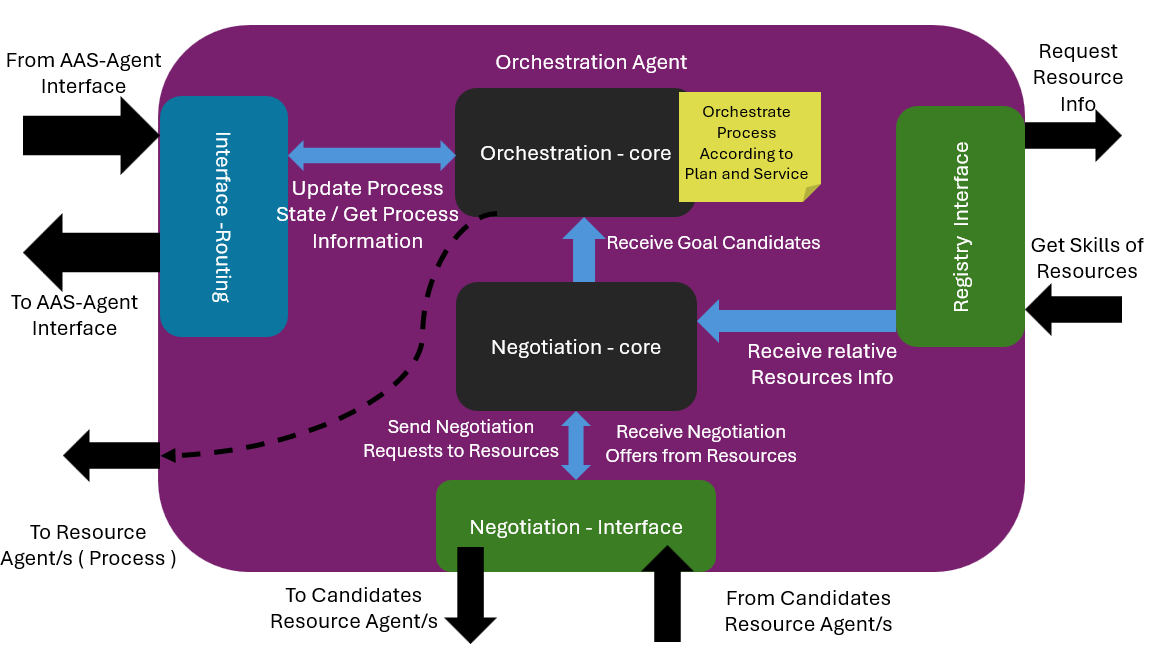
\includegraphics[width=0.99\textwidth]{Images/Production_Agent_Orchestration_Overview.png}
    \caption{Product AAS - Orchestration Agent and Negotiation Core}
    \label{fig:product_aas_orchestration_agent}
\end{figure}

As in figure \ref{fig:product_aas_orchestration_agent} the Orchestration Agent is the main component of the Product AAS where it contains the Orchestration Core and the Negotiation Core that represents the product in the system.
The Orchestration Core and the Negotiation Core are created via \textbf{SPADE} framework which is an open source framework for creating Multi-agent systems in python.
The Orchestration Core is responsible for managing the overall production process and coordinating the resources.
The Negotiation Core is responsible for negotiating with the Resource Agents to allocate the necessary resources for the production process.
The Orchestration Core and the Negotiation Core can also communicate with other agents in the system via XMPP protocol.

After landing a deal with the Resource Agents the Negotiation Core informs the Orchestration Core about the allocated resources.
The Orchestration Core then manages the production process using the allocated resources.
The Orchestration Core connects with the AAS-Agent Interface so that it can read and update the AAS Submodels.
The Orchestration Core also connects to other agents in the system via XMPP protocol.
The Orchestration Core can delegate tasks to the Negotiation Core so that it can focus on managing the production process.

The Negotiation Core also connects to the Registry Service so that it can discover the available Resource Agents in the system.
The Registry Service contains information about the available Resource Agents in the system including their capabilities and skills.
The Negotiation Core uses this information to negotiate with the Resource Agents to allocate the necessary resources for the production process.


\newpage
\section{System Components}
In this section, we delve into the various components that make up the AAS Type3 system architecture. Each component is described in terms of its functionality, interactions with other components, and its role within the overall system.

\subsection{Resource Agent Components}

\begin{figure}[ht]
    \centering
    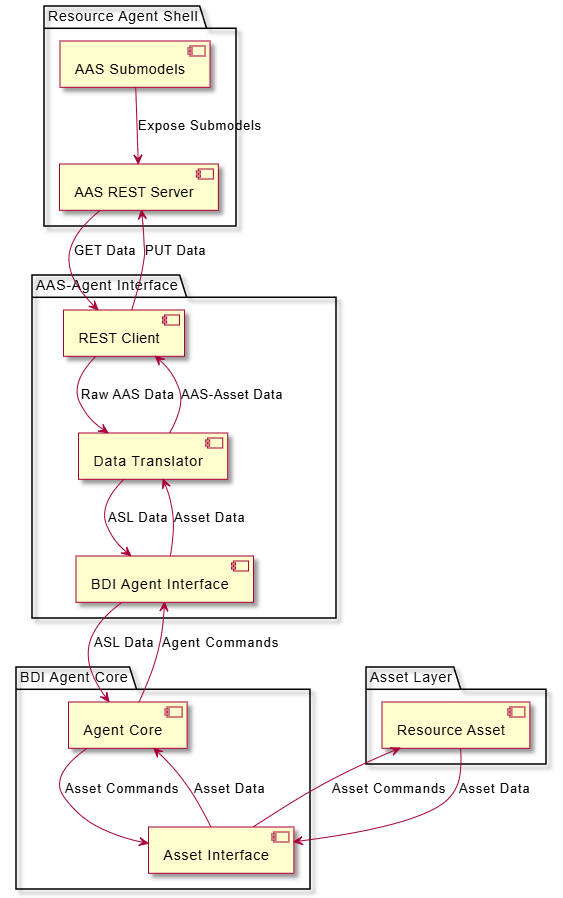
\includegraphics[width=0.7\textwidth]{Images/Resource_agent_components.png}
    \caption{Resource Agent Components Diagram}
    \label{fig:resource_agent_components}
\end{figure}

As illustrated in Figure \ref{fig:resource_agent_components}, the Resource Agent is composed of several key components over the layers that was discussed in the previous section.
In the first layer that is the \textbf{Resource Agent Shell}, it contains the following components:
\begin{itemize}
  \item \textbf{AAS Submodels} : those are the submodels of the AAS that describe the resource properties and capabilities.
  in which a Java server is used to host the AAS and provide access to its submodels.
  The server stores the AAS data into a database MongoDB for efficient retrieval and management.
  The AAS are mainly Json files that follow the AAS specification.
  \item \textbf{REST API server} : this component provides a RESTful interface for communication between the AAS and other system components.
  The Basyx framework provides this REST API server that allows clients to interact with the AAS submodels.
  The REST API server is a part of the Java server that hosts the AAS.
  It also opens MQTT communication channels for pub/sub messaging for real-time data exchange on update , create and delete operations on the AAS submodels. 
\end{itemize}

In the second layer that is the \textbf{AAS-Agent Interface layer}.
This layer as discussed before is responsible for the communication between the AAS and the Agent.
The layer contains three main components:
\begin{itemize}
  \item \textbf{REST Client} : This is the main layer for communication between the Agent and the AAS.
  Which is responsible for sending requests to the AAS REST API server and receiving responses.
  This client shall allow the Agent to read , write and deleted information about the asset, submodels and the submodels elements.
  \item \textbf{Data Translator} : This is the core component of the AAS-Agent interface layer.
  It is responsible for translating the data between the AAS format and the Agent's internal data structures.
  Where it takes raw data from the AAS and converts them into a format that the Agent can understand and vice versa.
  \item \textbf{BDI Agent Interface }: This component acts as a bridge between the Data Translator and the BDI Agent.
  It ensures that the translated data is properly integrated into the Agent's belief, desire, and intention structures.
  It also facilitates the communication of the Agent's decisions and actions back to the AAS through the Data Translator.
\end{itemize}
The last layer is the \textbf{BDI Agent Core} layer.
This layer contains the main components of the BDI Agent architecture:
\begin{itemize}
  \item \textbf{Agent Core} : This is the central component of the BDI Agent.
  It manages the Agent's beliefs, desires, and intentions.
  It processes incoming data from the AAS and makes decisions based on its internal state and goals.
  It also procees data coming from the Resource Asset it is assigned to manage.
  The main functionality is update beliefs based on the data received from the AAS and the Resource Asset.
  Then it generates desires and intentions based on the updated beliefs and the Agent's objectives.
  \item \textbf{Asset Interface} : This component is responsible for communication between the BDI Agent and the Resource Asset.
  It contains the necessary protocols and methods to interact with the asset, retrieve data, and send commands.
\end{itemize}

\newpage
\subsection{Production Agent Components}

\begin{figure}[ht]
    \centering
    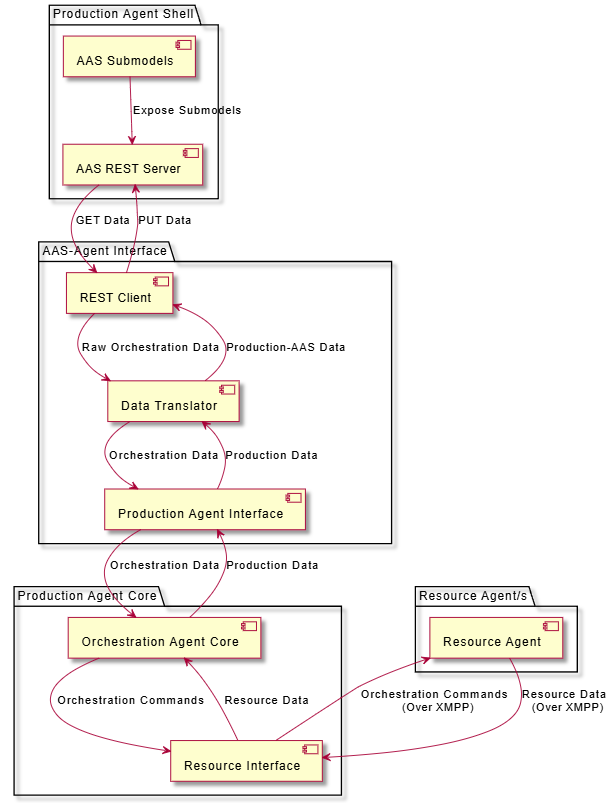
\includegraphics[width=0.8\textwidth]{Images/Production_Agent_Components.png}
    \caption{Production Agent Components Diagram}
    \label{fig:production_agent_components}
\end{figure}

The Production Agent components are illustrated in Figure \ref{fig:production_agent_components}.
It has similar structure to the Resource Agent components with some differences in the Agent Core layer and the AAS-Agent Interface layer.
In the \textbf{AAS-Agent Interface layer}, the components are similar to the Resource Agent with the data translator being adapted to handle production-specific data from the AAS submodels.
This includes translating production schedules, work orders, and status updates between the AAS format and the Agent's internal structures.
The AAS-Agent Interface gets the Raw orchestration commands from the Production AAS where it then translates them into an orchestration command
that the orchestration core can understand and act upon.
At the same time the data coming from the Production Agent core about the production status and progress is translated back into the AAS format and updated into the Production AAS submodels.

In the main layer that is the \textbf{Production Agent core} layer the diffrences are more significant.
The Production Agent core contains the \textbf{orchestration agent core } component instead of the BDI agent core.
This component is responsible for managing the orchestration of production tasks and workflows.
It processes orchestration commands received from the AAS-Agent interface layer and coordinates the execution of these
tasks across multiple Resource Agents and assets.
It also monitors the progress of production activities and updates the AAS with status information through the AAS-Agent interface layer.
The \textbf{Resource Interface} component in this layer is also adapted
to handle communication with production-related assets, such as manufacturing equipment and assembly lines.
It ensures that the Production Agent can effectively manage and control these assets as part of the overall production process.



\newpage
9\section{Classes and Objects}

In this section a breakdown of the main classes and objects used in the system architecture is provided. Each class is described in terms of its attributes, methods, and relationships with other classes.

\subsection{Resource AAS classes}
In this subsection a detailed breakdown of the classes representing the AAS-Agent interface , the BDI agent Layer and the defnition of the Submodels .

\newpage
\subsubsection{Submodels definition}
In this subsection is the definition of the submodels of the Resource AAS.
Figure \ref{fig:submodel_classes} shows the class diagram representing the Resource Submodel, while Table \ref{tab:submodels_overview} provides an overview of each submodel along with its elements and definitions.
\begin{figure}[htpb]
    \centering
    \includesvg[width=0.9\textwidth,inkscapelatex=false]{Images/Classes_Resource/Submodels/Submodels.svg}
    \caption{Class diagram representing the Resource Submodel.}
    \label{fig:submodel_classes}
\end{figure}

\begin{table}[ht]
  \centering
  \caption{Overview of Resource Submodels and their elements}
  \label{tab:submodels_overview}
  \begin{tabularx}{\textwidth}{|l|X|X|}
    \hline
    \textbf{Submodel} & \textbf{Elements} & \textbf{Definition / Purpose} \\
    \hline
    Operational State & Current State , Historical Data & Represents the current and historical operational states of the resource. \\
    \hline
    Knowledge & Resource Constraints, Environmental Conditions & Contains knowledge about resource constraints and environmental conditions affecting operations. \\
    \hline
    Capability & Drill , MoveXY ,Skill & Defines the capabilities and skills of the resource for task execution. \\
    \hline
    Interaction and Scheduling & Endpoints & Manages interaction points and scheduling information for resource coordination. \\
    \hline
  \end{tabularx}
\end{table}

\newpage
\subsubsection{REST Client}
This subsection provides a detailed breakdown of the classes representing the REST Client used for communication with the AAS.
Figure \ref{fig:rest_client_classes} shows the class diagram representing the REST Client.
\begin{figure}[ht]
    \centering
    \includesvg[width=0.9\textwidth,inkscapelatex=false]{Images/Classes_Resource/REST_Client.svg}
    \caption{Class diagram representing the REST Client.}
    \label{fig:rest_client_classes}
\end{figure}

The main design of this component is the two repository classes, the \emph{AAS Repository} class that is responsible for all the communication with the AAS over REST API calls, and the \emph{Submodel Repository} class that is responsible for all the communication with a specific submodel of the AAS over REST API calls.
Both classes use the \emph{HTTP Client} class that is a wrapper over the HTTP library used to perform the REST API calls.
Those then are called into the main class \emph{REST Client} that creates, starts, and stops a client session.
Also the class provides a simple MQTT client to subscribe to AAS events over MQTT protocol.
This client is represented by the \emph{AASEvent} class.

\newpage
\subsubsection{AAS-Agent Interface}
This subsection provides a detailed breakdown of the classes representing the AAS-Agent interface.
Figure \ref{fig:aas_agent_interface_classes} shows the class diagram representing the AAS-Agent Interface.
\begin{figure}[ht]
    \centering
    \includesvg[width=0.8\textwidth,inkscapelatex=false]{Images/Classes_Resource/DataTranslator.svg}
    \caption{Class diagram representing the AAS-Agent Interface.}
    \label{fig:aas_agent_interface_classes}
\end{figure}

This interface provides the needed datatypes to switch between the data coming from the AAS and the data coming from the Resource Asset over the agent.
The datatype that represent the data coming from the AAS to the agent is the \emph{AAS Data Model} class, while the datatype that represent the data coming from the Resource Asset to the agent is the \emph{Resource Data Model} class.
This conversion is done through the \emph{DataParser} class that is an abstract class that contains the methods needed for the conversion between the two datatypes.
The \emph{AAS to Resource Data Parser} class is a concrete implementation of the \emph{DataParser} class that implements the conversion from the \emph{AAS Data Model} to the \emph{Resource Data Model}, while the \emph{Resource to AAS Data Parser} class is a concrete implementation of the \emph{DataParser} class that implements the conversion from the \emph{Resource Data Model} to the \emph{AAS Data Model}.
Finally the \emph{Data Translator} is the main level that is callable through entry points from the BDI agent layer to perform the needed conversion between the two datatypes.
In the lowest level there is two enums  the \emph{AAS Data Types} enum that contains the data types used in the AAS Data Model and the \emph{Resource Data Types} enum that contains the data types used in the Resource Data Model.

\newpage
\subsubsection{BDI Agent Core}
This subsection provides a detailed breakdown of the classes representing the BDI Agent Core.
Figure \ref{fig:bdi_agent_core_classes} shows the class diagram representing the BDI Agent Core.
\begin{figure}[ht]
    \centering
    \includesvg[width=0.9\textwidth,inkscapelatex=false]{Images/Classes_Resource/BDI_Core/Agent_core.svg}
    \caption{Class diagram representing the BDI Agent Core.}
    \label{fig:bdi_agent_core_classes}
\end{figure}

By using \textbf{SPADE} framework , there is an architecture that represents the BDI agent core.
Mainly each agent core contians an Agent core where the BDI Agent lives and Behaviours that represent the different functionalities of the agent.
In the figure \ref{fig:bdi_agent_core_classes} is the Agent Core represented ,while in figure \ref{fig:bdi_agent_behaviours_classes} are the different behaviours of the agent represented.
\begin{figure}[ht]
    \centering
    \includesvg[width=0.95\textwidth,inkscapelatex=false]{Images/Classes_Resource/BDI_Core/Behaviours.svg}
    \caption{Class diagram representing the BDI Agent Behaviours.}
    \label{fig:bdi_agent_behaviours_classes}
\end{figure}

The \emph{ResourceAgent} class is the main class that represents the BDI agent.
Its mainly an implementation of the \textbf{SPADE} \emph{BDIAgent} class.
The needed methods to be implemented are the \emph{setup} method that is called when the agent is started and the \emph{add custom actions} that let the agent define action or desires that is represtented in the behaviours.
The Data exchange between the agents in the \textbf{SPADE} framework is done mainly throgh \textbf{Templates} which are represented by the \emph{Resource Agent Templates} class.
The Behaviours of the agent is represented by two abstract classes of the \textbf{SPADE} framework: \emph{OneShotBehaviour} and \emph{CyclicBehaviour}.
Those then are implemented into different concrete classes like the \emph{Proposal Process Behaviour} class that is responsible for handling the proposals coming from the Orchestrator agent, the \emph{Task Execution Behaviour} class that is responsible for executing the tasks assigned to the resource, and the \emph{Status Update Behaviour} class that is responsible for updating the status of the resource in the AAS at regular intervals.

\newpage
\subsection{Production AAS classes}
This subsection provides a detailed breakdown of the classes representing the Production AAS-Agent interface , the Orchestrator Layer and the definition of the Submodels.

\subsubsection{Submodels definition}

In this subsection is the definition of the submodels of the Production AAS.
Figure \ref{fig:prod_submodel_classes} shows the class diagram representing the Production Sub
model, while Table \ref{tab:prod_submodels_overview} provides an overview of each submodel along with its elements and definitions.
\begin{figure}[ht]  
    \centering
    \includesvg[width=0.7\textwidth,inkscapelatex=false]{Images/Production_Classes/Submodels.svg}
    \caption{Class diagram representing the Production Submodel.}
    \label{fig:prod_submodel_classes}
\end{figure}

\begin{center}
\begin{longtable}{|p{0.18\textwidth}|p{0.41\textwidth}|p{0.41\textwidth}|}
\caption{Overview of Production Submodels and their elements}
\label{tab:prod_submodels_overview}\\
\hline
\textbf{Submodel} & \textbf{Elements} & \textbf{Definition / Purpose} \\
\hline
\endfirsthead
\multicolumn{3}{c}{\tablename\ \thetable\ -- \textit{Continued from previous page}} \\
\hline
\textbf{Submodel} & \textbf{Elements} & \textbf{Definition / Purpose} \\
\hline
\endhead
\hline \multicolumn{3}{r}{\textit{Continued on next page}} \\
\endfoot
\hline
\endlastfoot
Process Plan & Entry \& Exit; Nodes; Edges; Preconditions; Postconditions; Required Input \& Output; Required Capabilities. & Defines the procedural/workflow model for a production task. Nodes represent steps, edges represent transitions; pre/postconditions control applicability; inputs/outputs and required capabilities describe data and resources needed by each step. Used for orchestration and execution planning. \\
\hline
Services Catalog & Services (service id, signature, parameters, category). & Registry of callable services / functional capabilities exposed by the production component. Describes available service operations, required parameters and invocation metadata for integration and discovery. \\
\hline
Execution State \& Tracking & Timestamps; Token position; Current node; Step status; Measured parameters. & Runtime information about process execution and monitoring: timestamps and token positions for traceability, current node and step status for progress reporting, measured parameters for quality/telemetry. Enables tracking, auditing and recovery. \\
\hline
Interface and Endpoints & SkillCall Endpoints (URIs / endpoint descriptors). & Communication and integration endpoints used to invoke skills or services remotely (e.g., orchestrator calls, skill invocation). Contains addressing and protocol metadata for external interaction. \\
\hline
Header / Metadata & idShort, id, administration/asset information, semantic identifiers, versioning. & Global AAS header and identification information that links the submodel to the asset and provides administrative metadata (identifiers, semantic references and versioning). Used for discovery and semantic alignment. \\
\hline
\end{longtable}
\end{center}

\newpage
\subsubsection{REST Client}
Similar to the Resource AAS REST client, this subsection provides a detailed breakdown of the classes representing the REST Client used for communication with the Production AAS.
Figure \ref{fig:prod_rest_client_classes} shows the class diagram representing the REST Client.
\begin{figure}[ht]
    \centering  
    \includesvg[width=0.99\textwidth,inkscapelatex=false]{Images/Production_Classes/Client.svg}
    \caption{Class diagram representing the REST Client.}
    \label{fig:prod_rest_client_classes}
\end{figure}
The design of this component is similar to the Resource AAS REST client, with two repository classes: the \emph{Production AAS Repository} class for communication with the Production AAS over REST API calls, and the \emph{Production Submodel Repository} class for communication with specific submodels of the Production AAS over REST API calls.
Both classes utilize the \emph{HTTP Client} class for performing REST API calls.
The main class \emph{REST Client} creates, starts, and stops a client session, and also provides an MQTT client to subscribe to Production AAS events over the MQTT protocol, represented by the \emph{ProductionAASEvent} class.


\newpage
\subsubsection{AAS-Agent Interface}
This subsection provides a detailed breakdown of the classes representing the Production AAS-Agent interface.
Figure \ref{fig:prod_aas_agent_Translator_classes} shows the class diagram representing the Production AAS-Agent Interface.
\begin{figure}[ht]
    \centering  
    \includesvg[width=0.8\textwidth,inkscapelatex=false]{Images/Production_Classes/Translator.svg}
    \caption{Class diagram representing the Production AAS-Agent Interface.}
    \label{fig:prod_aas_agent_Translator_classes}
\end{figure}

The main diffrerence between this interface and the Resource AAS-Agent interface is the datatypes used.
The datatype that represent the data coming from the Production AAS to the Orchestrator agent is the \emph{Production AAS Data Model} class, while the datatype that represent the data used internally by the Orchestrator agent is the \emph{Production Data Model} class.
This conversion is done through the \emph{Production DataParser} class that is an abstract class that contains the methods needed for the conversion between the two datatypes.
The \emph{Production AAS to Production Data Parser} class is a concrete implementation of the \emph{Production DataParser} class that implements the conversion from the \emph{Production AAS Data Model} class to the \emph{Production Data Model} class.
The Interface is showen in figure \ref{fig:prod_aas_agent_interface_classes}.
\begin{figure}[ht]
    \centering  
    \includesvg[width=0.8\textwidth,inkscapelatex=false]{Images/Production_Classes/Interface.svg}
    \caption{Class diagram representing the Production AAS-Agent Interface.}
    \label{fig:prod_aas_agent_interface_classes}
\end{figure}

\newpage
\subsubsection{Orchestration and Negotiation Core}

This subsection provides a detailed breakdown of the classes representing the Orchestration and Negotiation Core.
The orchestration Core is represented in figure \ref{fig:orchestration_core_classes}.
\begin{figure}[ht]
    \centering  
    \includesvg[width=0.9\textwidth,inkscapelatex=false]{Images/Production_Classes/Agent_Core/Orch_Core.svg}
    \caption{Class diagram representing the Orchestration Core.}
    \label{fig:orchestration_core_classes}
\end{figure}
The Orchstrator is the main class that represents the Orchestrator agent.
Its mainly an implementation of the \textbf{SPADE} \emph{Agent} class.
The needed methods to be implemented are the \emph{setup} method that is called when the agent is started and the \emph{add custom actions} that let the agent define action or desires that is represtented in the behaviours.
The Data exchange between the agents in the \textbf{SPADE} framework is done mainly throgh \textbf{Templates} which are represented by the \emph{Orchestrator Agent Templates} class.
The Behaviours of the agent is represented by an abstract classe of the \textbf{SPADE} framework: \emph{OneShotBehaviour}.
Those then are implemented into different concrete classes like the \emph{Allocate Skill To Resource Behaviour} class that is responsible for allocating skills to resources based on their capabilities, and the \emph{Negotiation Behaviour} class that is responsible for handling the negotiation process with Resource agents to finalize task assignments.

The other core which is the Negotiation core is represented in figure \ref{fig:negotiation_core_classes}.
This is also represented by and Agent class in the \textbf{SPADE} framework.
It also have defined behaviours that are represented in the figure. \ref{fig:negotiation_core_classes}.
\begin{figure}[ht]
    \centering
    \includesvg[width=0.9\textwidth,inkscapelatex=false]{Images/Production_Classes/Agent_Core/Negotiation_Core.svg}
    \caption{Class diagram representing the Negotiation Core.}
    \label{fig:negotiation_core_classes}
\end{figure}

The two cores work together to manage the orchestration of production tasks and the negotiation with Resource agents to ensure optimal task assignments based on resource capabilities and time availability.



\newpage
\section{Flows and State Machines}

TBD .

\bibliographystyle{IEEEtran}
\bibliography{references}
\end{document}